\chapter{Softwarearchitektur}
Softwarearchitektur beschäftigt sich im Wesentlichen mit dem Erstellen des Fundamentes eines Softwaresystems. Der Fokus liegt nicht auf Implementationsdetails sondern auf Strukturen, logischen und physischen Komponenten, Beziehungen und Schnittstellen. \cite[S. 9-10]{softarch}

Durch diese Abstraktionen wird versucht, die Komplexität des Systems \glqq überschaubar und handhabbar\grqq \cite[S. 10]{softarch} zu machen, um so früh wie möglich Risiken und Probleme zu identifizieren und die Qualität der zu erstellenden Software zu sichern. \cite[S. 10]{softarch}

Diese einzelnen Abstraktionen können in Architektursichten gruppiert werden.

\section{Architektursichten}
Architektursichten beschreiben verschiedene Sichten auf das zu erstellende System und entstanden in den späten 80ern bzw. frühen 90ern. Im Jahre 2000 wurde schließlich eine Empfehlung zur Erstellung von Softwarearchitektur vom Institute of Electronics Engineers (IEEE 1471) heraus gegeben, in welchem Architektursichten erwähnt, aber weder Sichtenmodelle noch Modellierungssprachen festgelegt werden \cite{ISO_ARCH_OLD}\cite[S. 138]{basiswissen}. Die Empfehlung wurde im Jahre 2011 von der ISO unter der Nummer 42010 standardisiert\cite{ISO_ARCH}.

ISO 42010 definiert eine Architektursicht folgendermaßen: Eine Architektursicht ist eine Sicht der Architektur eines Systems aus der Perspektive von ein oder mehreren Stakeholdern. Diese Stakeholder haben unterschiedliche Aufgaben und Interessen und benötigen somit auf ihre Bedürfnisse zugeschnittene Information. Die einzelnen Sichten wiederum beinhaltet mehrere Architekturmodelle. \cite{ISO_ARCH}

Ein Beispiel für einen Stakeholder ist zB. ein/eine SystementwicklerIn. Sie/Er benötigt für das Aufsetzen und Konfigurieren der Hardwarekomponenten eine Sicht auf die physische Verteilung des Systems. Diese Sicht kann zB. mit Hilfe des UML Komponentendiagramms beschrieben werden. Das Komponentendiagramm nimmt hier die Rolle des Architekturmodells an.

\section{Architektursichtenmodelle}
ISO 42010 definiert, wie erwähnt, weder Architektursichten- noch Architekturmodelle, stellt jedoch einen Rahmen für diese bereit
\cite[S. 138]{basiswissen}. Diese können, je nach Bedürfnissen der ArchitektInnen, aus einer großen Anzahl von Architektursichtenmodellen ausgewählt werden. \cite[S. 142-145]{basiswissen}

Folgende Architektursichtenmodelle werden häufig verwendet \cite[S. 94]{softarch}:

\begin{itemize}
  \item Zachmann Framework
  \item RM-ODP
  \item Kruchtens 4+1 Sichtenmodell
\end{itemize}

Das Zachmann Framework, benannt nach dessen Autor John Zachmann, geht auf den Versuch zurück, Strukturen von Unternehmen zu beschreiben. Das Modell wurde später für Softwarearchitekturen abgewandelt. Das Framework eignet sich vor allem für Enterprisesysteme, da die Organisation des Unternehmens gut beschrieben werden kann. Für andere Einsatzfälle wird jedoch aufgrund der Komplexität empfohlen, das Modell einzuschränken. \cite[S. 94-95]{softarch}

RM-ODP, kurz für Reference Model for Open Distributed Processing, ist ein von der ISO standardisiertes Architektursichtenmodell, welches sich vor allem für verteilte, objektbasierte Systeme eignet. Es versucht vor allem Architekturen unabhängig \glqq von Verteilungs- und Verteilungsaspekten\grqq zu machen. \cite{ISO_RMODP}\cite[S. 97-98]{softarch}

Das 4+1 Schichtenmodell, welches von Philipp Kruchten entwickelt wurde, fokussiert vor allem die Stakeholder ProjektmanagerInnen, EntwicklerInnen und BenutzerInnen. Das Modell beinhaltet folgende Sichten \cite{kruch}\cite[S. 501-503]{appluml}:

\begin{itemize}
  \item Logical View: Logische Sicht auf das System, welche sich mit der Funktionalität des Systems beschäftigt. Kann durch UML Paket-, Klassen- und Interaktionsübersichtsdiagramme beschrieben werden.
  \item Process View: Beschäftigt sich mit dem Laufzeitverhalten des Systems, wie zB. Prozessen, Parallelität und Kommunikation. UML Klassen- und Interaktionsübersichtsdiagramme können hierfür verwendet werden.
  \item Development View: Beschreibt die Aufteilung des Systems in Module und Bibliotheken aus der Sicht des Programmierers. Kann durch UML Paket- und Komponentendiagramme beschrieben werden.
  \item Physical View: Regelt und beschreibt die Verteilung der Komponenten auf physische Systeme. UML Komponenten- und Verteilungsdiagramm bieten sich hierfür an.
  \item Scenarios: Beschreibt die Usecases eines Systems, um die Architekturentscheidungen zu validieren. Hierfür können UML Usecasediagramme verwendet werden.
\end{itemize}

In der Arbeit wird vor allem auf Kruchtens 4+1 Sichtenmodell eingegangen. Aufgrund der Einschränkung auf die Planungsphase der Architektur entfallen jedoch diverse Sichten. Dies sind vor Allem jene, welche stark auf die Implementierung fixiert sind, zB. die Process View.

\section{Architekturprozess Lifecycle}
Zeitlich ordnet sich die Architekturphase zwischen dem Ermitteln der Anforderungen und der tatsächlichen Implementation ein. Da die Erstellung von Software heutzutage mehr ein agiler und inkrementeller Prozess ist, wird auch die Erstellung und die Mitwirkung der Softwarearchitektur in diese sich wiederholenden Prozesse mit einbezogen. \cite[S. 7]{basiswissen}

Der Architekturzyklus lässt sich mit dem in Abbildung \ref{fig:cycle} beschriebenen Aktivitätsdiagramm darstellen und unterteilt sich in folgende Unterbereiche \cite[Umschlag]{softarch}:

\begin{itemize}
  \item \glqq Erstellen der Systemvision\grqq
  \item \glqq Verstehen der Anforderungen\grqq
  \item \glqq Entwerfen der Architektur\grqq
  \item \glqq Umsetzen der Architektur\grqq
  \item \glqq Kommunizieren der Architektur\grqq
\end{itemize}

Die Systemvision beschreibt die Grundidee des zu erstellenden Systems. Sie geht meist vom/von der KundIn aus und wird am Anfang des Projektes erstellt. Eine Systemvision beinhaltet die Antwort auf folgende drei Punkte \cite[S. 202-206]{vision}:

\begin{itemize}
  \item Was soll das Projekt erreichen?
  \item Warum ist es wertvoll?
  \item Was sind die Kriterien, welche den Erfolg des Projekt beeinflussen?
\end{itemize}

Bereits hier sollte ein/eine SoftwarearchitektIn anwesend sein, um die Anforderungen zu prüfen, die Machbarkeit zu ermitteln und auf widersprüchliche Anforderungen hinzuweisen. \cite[S. 352-353]{softarch}

Ist die Systemvision erstellt und die Anforderungen ermittelt, müssen diese in eine Form gebracht werden, welche widerspruchsfrei und klar ist. Unpräzise Anforderungen müssen präzisiert werden. Oft findet auch eine Priorisierung der Anforderungen statt. \cite[S. 353]{softarch}

Danach kann mit der Planung der Architektur begonnen werden. Die Anforderungen liefern die Basis für die architektonischen Entscheidungen. In dieser Phase findet meist auch ein Architekturreview statt, um Alternativarchitekturen abzuwägen. \cite[S. 353]{softarch}

Steht die Planung der Architektur wird schließlich mit der Implementation begonnen. Hier muss darauf geachtet werden, dass die architektonischen Entscheidungen korrekt umgesetzt werden, da diese erfahrunsgemäß oft vernachlässigt werden. \cite[S. 354]{softarch}

Während der Architekturphase müssen die Entscheidungen des Architekturprozesses kontinuierlich den Stakeholdern kommuniziert werden, damit diese die Architektur umsetzen und bei auftretenden Problemen Feedback geben können. \cite[S. 354]{softarch}

\begin{figure}[H]
    \centering
    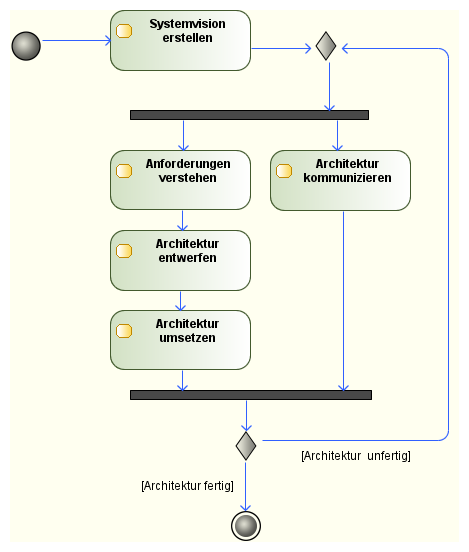
\includegraphics[scale=0.6]{img/archcycle.png}
    \caption{Der Architekturprozess modelliert als Aktivitätsdiagramm \cite[Umschlag, S. 352]{softarch}}
    \label{fig:cycle}
\end{figure}

Der Fokus der Arbeit liegt wegen der fehlenden Implementierung hauptsächlich auf den ersten drei Teilen, der Erstellung der Systemvision, Verstehen der Anforderungen und dem Entwerfen der Architektur.

\section{Was macht eine gute Softwarearchitektur aus}
Die Frage, was eine gute Softwarearchitektur ausmacht, wird oft sehr breit und ungenau beantwortet: Eine gute Architektur erfülle die \glqq Verhaltens-, Qualitäts- und Lebenszyklusanforderungen\grqq \ \cite[S. 12]{basiswissen} eine Systems, ermögliche es Risiken frühzeitig zu erkennen und die inhärente Komplexität eines Systems und dessen Quellcodes zu beherrschen \cite[S. 7-8]{softarch}.

Alle diese Kriterien lassen sich jedoch schwierig oder gar nicht messen. Manche Werte sind zwar messbar, aber lassen keine eindeutigen Entscheidungen ableiten: zB. können Kopplung und Kohäsion eines Systemes gemssen werden, jedoch kann nicht eindeutig festgelegt werden, ab welchem Wert die Kopplung zu hoch oder die Kohäsion zu niedrig ist.

Dieter Masek kommt zu folgendem Schluss: \glqq Die Frage ob eine gegebene Architektur gut oder schlecht ist, lässt sich nicht direkt beantworten. Gut oder schlecht sind absolute Bewertungen, die für Architekturen sowieso nicht möglich sind. Eine Architektur lässt sich nur in einem festgelegten Kontext beurteilen d.h.: Wie gut löst eine Architektur ein vorgegebenes Problem? Selbst diese eingeschränkte Frage lässt sich nicht mit gut oder schlecht beantworten! \grqq \ \cite[S. 19]{review}

Trotz all dieser Probleme lassen sich dennoch Werte messen und überprüfen \cite[S. 19]{review}, welche in Verbindung mit unzureichenden Architektureintscheidungen gebracht werden können. Dies erlaubt folgenden Schluss: Die Ausgangsfrage, was eine gute Softwarearchitektur ausmacht, führt zu keiner Erkenntnis und ist damit mehr oder minder nutzlos: Es kommt nicht darauf an, ob eine Architektur gut ist, sondern ob eine Architektur die an sie gestellten Anforderungen erfüllt.

Viele dieser Anforderungen stehen im Gegensatz zueinander: zB. erfordert eine hohe Performance eine niedrigere Abstraktionsebene, was jedoch die Wartung des Codes erschwert. Die Findung einer angemessene Softwarearchitektur beschäftigt sich somit mehr mit der Abwägung von Vor- und Nachteilen, welche aus den jeweiligen Entwurfsmustern und Technologien ableitbar sind.

Um diese Entscheidungen abwägen zu können, ist wichtig, die expliziten Anforderungen an das System zu kennen \cite[S. 19]{review}. Eine möglichst vollständige Anforderungsanalyse ist somit die Ausgangsbasis für eine angemessene Softwarearchitektur. Dies kann jedoch vor allem am Anfang der Anforderungsanalyse schwierig sein, da die KundInnen noch keine genaue Vorstellung vom zu entwickelnden System haben \cite[S. 80]{reqman}.

Eine Möglichkeit zur Überprüfung von bestehenden und noch nicht beachteteten Anforderungen der Architektur stellt die Durchführung eines szenariobasierten Architekturreviews wie ATAM oder CBAM dar.


\section{Architekturbewertungsmethoden}
Architekturbewertungsmethoden werden dazu verwendet, die Angemessenheit einer Architektur zu überprüfen. Die Meisten ihrer Art basieren auf der Erstellung von Szenarien, da das Kosten-Nutzen Verhältnis dieser Herangehensweise sehr gut ist \cite[S. 185]{basiswissen}.

Es gibt mehrere verschiedene Bewertungsmethoden wie CBAM, ALMA und ARID, welche zum Großteil Abwandlungen von ATAM darstellen. ATAM wiederum ist eine Weiterentwicklung von SAAM. \cite[S. 60-76]{review}

Da Kosteneffektivität, Änderungs- und Wachstumsszenarien die Basis für Entscheidungen des erstellten Architekturprozesses darstellen, wird näher auf ATAM (Änderungs- und Wachstumsszenarien) und CBAM (Kostenszenarien) eingegangen.

\subsection{ATAM}
ATAM, kurz für Architecture Trade-off Analysis Method, beschäftigt sich mit den nicht funktionalen Anforderungen wie Performance oder Verfügbarkeit. Sie lässt sich in folgende Phasen einteilen \cite[S. 185]{basiswissen}:

\begin{itemize}
  \item Vorbereitungsphase
  \item Architekturzentrierte Bewertung
  \item StakeholderInnenzentrierte Bewertung
  \item Nachbearbeitungsphase
\end{itemize}

Einer initialen Vorbereitungsphase, in welchem das Team und der Zeitplan erstellt wird, folgt ein Treffen mit den StakeholderInnen des/der AuftraggeberIn, in der die Geschäftsziele und Architektur vorgestellt werden. In diesem Treffen werden die nicht funktionalen Anforderungen anhand eines Utility Trees (Abbildung \ref{fig:utility}) erarbeitet, priorisiert und bewertet. Sind wichtige architekturrelevante Anforderungen noch nicht bekannt, können diese nun mit den StakeholderInnen erarbeit werden. \cite[S. 184-199]{basiswissen}

Der Utility Tree ist ein Baumstruktur, deren Blätter die nicht funktionalen Anforderungen sind. Diese nicht funktionalen Anforderungen werden danach in weitere, konkrete Unterbereiche aufgespalten, zB. Performance würde in Antwortzeit und Speicherbedarf aufgespaltet werden. Diese Unterbereiche können schließlich bewertet und priorisiert werden.

\begin{figure}[H]
    \centering
    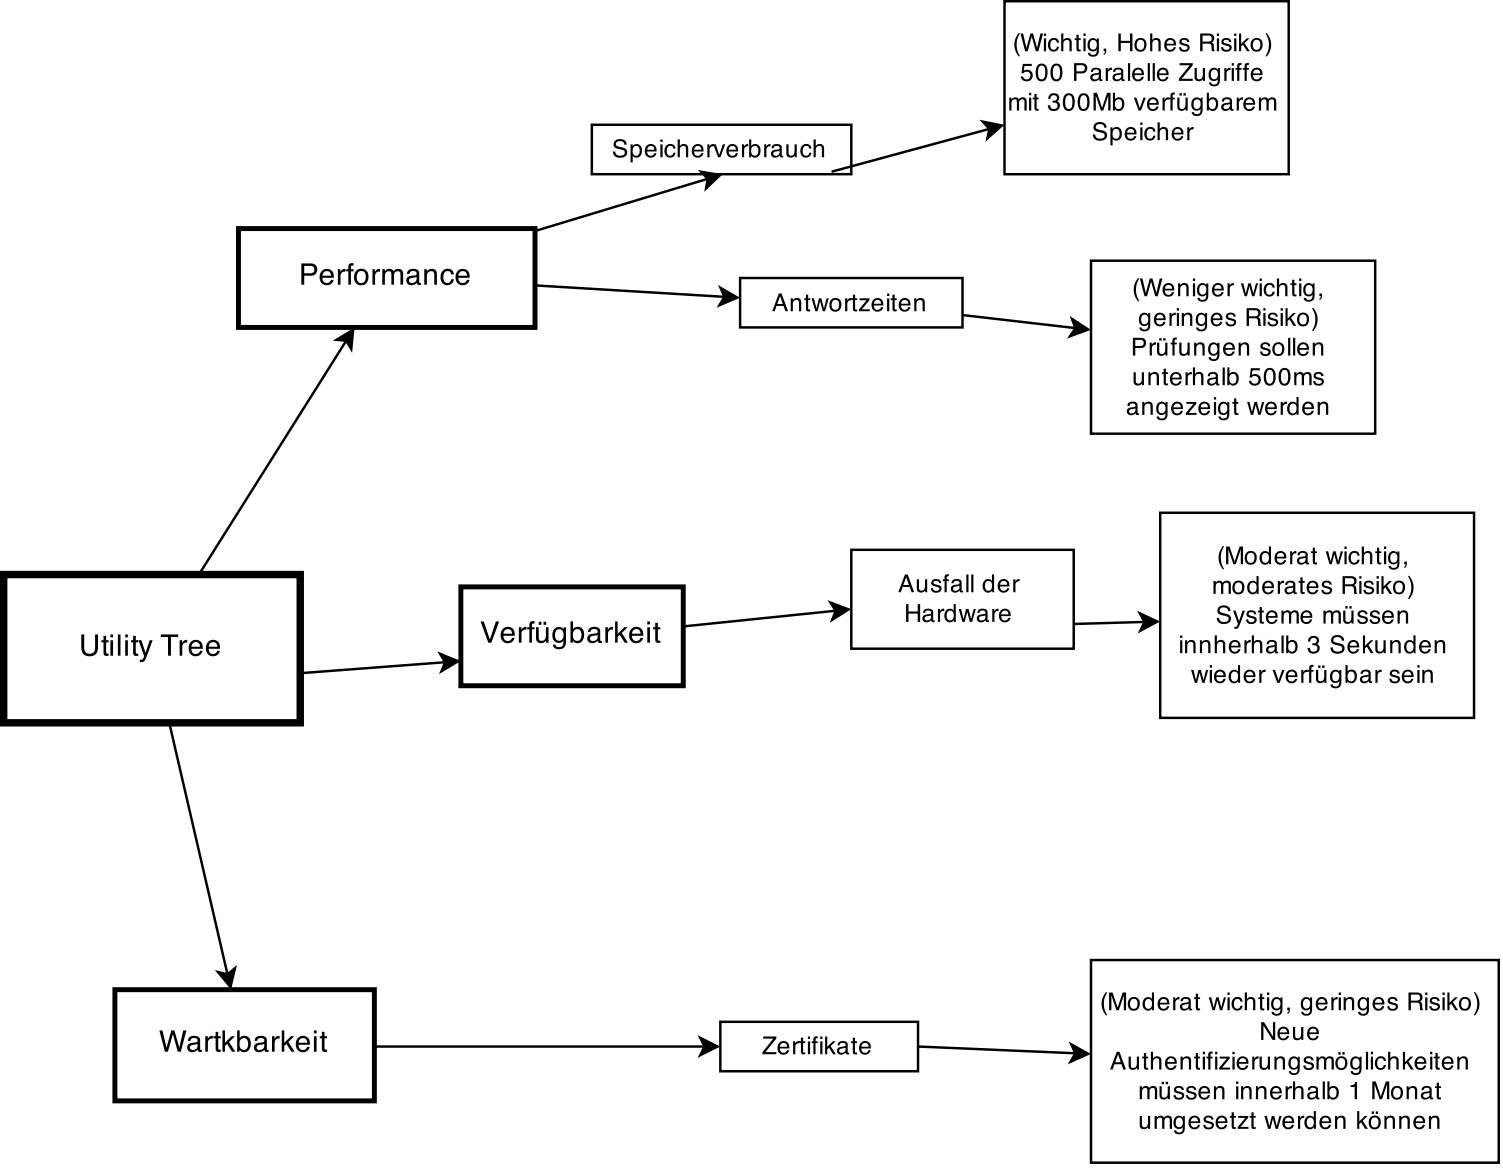
\includegraphics[scale=0.4]{img/utilitytree.png}
    \caption{Beispiel eines Utility Trees \cite[S. 17]{ATAM}}
    \label{fig:utility}
\end{figure}

Auf Basis des Utility Trees und dessen nicht funktionale Anforderungen werden dann in den darauf folgenden Bewertungsphasen folgende Szenarientypen überprüft \cite[S. 62-67]{review}\cite[S. 188]{basiswissen}:

\begin{itemize}
  \item Usecases
  \item Wachstumsszenarien
  \item Explorative Szenarien
\end{itemize}

Die Usecases beschreiben die Standardanwendungsfälle der NutzerInnen, welche durch das System umgesetzt werden sollen. Wachstumsszenarien beschreiben Szenarien, welche sich vor allem mit der Skalierbarkeit der Applikation beschäftigen, zB. statt 10 UserInnen greifen auf einmal 100 UserInnen auf das System zu. Explorative Szenarien drehen sich um mögliche Nutzungsszenarien, welche im Vorfeld entweder nicht bedacht wurden, oder nicht der Hauptfokus des Systems sind. \cite[S. 63]{review}

Alle Szenarien werden priorisiert. Danach führen die ArchtektInnen pro Usecase eine Analyse der im Utilitytree beschriebenen nicht funktionalen Anforderungen durch. Je nachdem, wie viel Zeit für die Analyse aufgewendet werden soll, werden zusätzlich zu den als hoch priorisierten Usecases und nicht funktionalen Anforderungen auch weitere, niedriger Priorisierte überprüft. \cite[S. 192]{basiswissen}

Sind die Bewertungsphasen abgeschlossen können die Ergebnisse analysiert, dokumentiert und präsentiert werden. Dies dient nicht nur als Dokumentation der geplanten Verbesserungen für die Architekturplanung, sondern hilft auch in zukünftigen ATAM Analysen die Entscheidungen früherer Analysen nachzuvollziehen. \cite[S. 189]{basiswissen}

\subsection{CBAM}

Eine Architektur ist meist nicht nur durch die ihr abverlangten Qualitätsanforderungen begrenzt, sondern auch durch die ihr zur Verfügung stehenden Mittel. Es mag zB. besser sein, eine hohe Kohäsion einer Komponente zu verlangen, um die Wartungskosten zu verringern, jedoch kann dies in manchen Fällen zu zu hohen Anschaffungskosten führen, da zB. statt einem Server zehn Server angeschafft werden müssen. Um die Kosten verschiedener Architekturen besser bewerten zu können, wurde CBAM entwickelt . CBAM, kurz für Cost Benefit Analysis Method, baut auf ATAM auf und ergänzt es um eine Kosten-Nutzen Analyse. Hauptkriterium dieser Analyse ist der ROI. \cite[S. 67-68]{review}

CBAM gliedert sich in folgende Phasen: \cite[S. 68]{review}

\begin{itemize}
  \item \glqq Triagephase\grqq
  \item \glqq Detailphase\grqq
  \item \glqq Attributsquantitfizierungsphase\grqq
  \item \glqq Kostenquantitfizierungsphase\grqq
  \item \glqq Rankingphase\grqq
\end{itemize}

In der Triagephase werden die möglichen Architekturen anhand ihrer Kosten und Vorteile grob bewertet. Die Bewertungen liefern dann die Grundlage für die Auswahl der möglichen Architektur(en). Bevorzugt wird die Architektur, welche die größt möglichsten Wertschöpfung erlaubt, sprich welche den ROI maximiert. \cite[S. 68]{review}

In der darauf folgenden Detailphase wird dann die ausgewählte Architektur und deren Qualitätsanforderungen genauer analysiert, um in der Attributsquantitfizierungsphase eine Aussage über die Auswirkungen auf die Qualitätsanforderungen treffen zu können. In der Kostenquantitfizierungsphase wird dann der ROI der verbleibenden Architekturen berechnet. \cite[S. 68-69]{review}

Abschließend wird dann auf Basis des ROI versucht, die Architektur mit dem größten ROI zu finden, welche das Budget für das System erlaubt. Im Gegensatz zu ATAM wird kein Utility Tree verwendet, sondern eine \glqq Utility-Response-Kurve\grqq, welche Auskunft über die Wirtschaftlichkeit der Qualitätsanforderungen liefert.  \cite[S. 69]{review}